\documentclass[english]{presentation}
%\setbeameroption{show notes on second screen}
%\setbeameroption{show only notes}

\usepackage{chngpage}
\usepackage{array}
\usepackage{tabularx}

% Presento style file
\usepackage{presento}

% strikethrough text
\usepackage[normalem]{ulem}

% macros
\usepackage{mama}

\renewcommand{\O}{\mathcal{O}}
\newcommand{\M}{\mathcal{M}}
\newcommand{\aetop}{\text{a.e.}}
\newcommand{\msbl}{\mathsf{msbl}}

\newcommand{\gold}[1]{{\color{colorgold}{#1}}}

\newcolumntype{C}{>{\centering\arraybackslash}X}

\renewcommand<>{\sout}[1]{%
	\alt#2{\beameroriginal{\sout}{#1}}{#1}%
}

\AtBeginDocument{%
 \abovedisplayskip=1ex
 \belowdisplayskip=1ex
 \abovedisplayshortskip=0pt
 \belowdisplayshortskip=7pt minus 4pt
}

\addbibresource{./bibliography.bib}

\title{My name is\\[-.8ex]\gold{stochastic calculus}\\[-.8ex]but everybody calls me\\[.2ex]\gold{calculus}}
%\subtitle{A TallCats talk}
\author{Matteo Capucci}
\institute{University of Strathclyde}
\date{March 11th, 2021\\(Day 434 of the COVID Era)}

\begin{document}
	\begin{frame}[plain]
		\maketitle
	\end{frame}

	\begin{frame}{Idea}
	\begin{center}
		
\includegraphics[width=\columnwidth]{figures/intro.png}
	\end{center}
	Something's going on...
\end{frame}

\begin{frame}{Preliminaries}
	Let's fix a probability space $W = (W, \F, \P)$.
	Recall that
	\begin{itemize}
		\item $W : \Set$\\
		Space of `outcomes' of a stochastic experiment
		\item $\F : \sigma$-field\\
		Space of `events', i.e. $\sigma$-algebra of subsets of $W$
		\item $\P : \F \to \R^+$\\
		'Probability measure', i.e. an assignment of beliefs to events
	\end{itemize}
	\begin{center}
		
\includegraphics[width=.5\columnwidth]{figures/proba-space.png}
	\end{center}
\end{frame}

\begin{frame}{Preliminaries}
	We call
	\begin{equation*}
		\ker \P = \{A \in \F \suchthat \P(A) = 0 \}
	\end{equation*}
	the $\sigma$-ideal of null sets.

	Let $V = (V, \G, \Q)$.
	\begin{center}
		\text{\underline{measurable maps}}\\
		$\Msbl(W, V) = \{ f : W \to V \suchthat f^{-1}\G \subseteq \F\}$\\[2ex]

		\text{\underline{null-reflecting maps}}\\
		$\Msbl_0(W, V) = \{ f \in \Msbl(W, V) \suchthat f^{-1}\ker\Q \subseteq \ker \P\}$
	\end{center}
\end{frame}

\begin{frame}{Preliminaries}
	\begin{definition}
		An $E$-valued \textbf{stochastic process} on $W$ is a collection of measurable maps
		\begin{equation*}
			X_t : W \to E, \qquad t \in I
		\end{equation*}
		where $I$ is a poset of \textbf{time}s and $E$ is a measurable space of \textbf{values}.
	\end{definition}

	\begin{example}
		Toss a coin and bet $1\$$ on heads: $W = \{H,T\}^\N$, $E = \R$, $I = \N$,
		\begin{equation*}
			X_n(\omega) = \sum_{i=0}^n (\delta^{\omega_i}_H(\omega) - \delta^{\omega_i}_T(\omega))
		\end{equation*}
	\end{example}
	\vspace{-3ex}
	\begin{example}
		You have a financial portfolio, your profit are a stochastic process $X_t$ which is a function of another stochastic process $M_t$, the market.
	\end{example}
\end{frame}

\begin{frame}{Preliminaries}
	A central concept in stochastic calculus is that of filtration:
	\begin{definition}
		A \textbf{filtration} on $W$ is a sequence of $\sigma$-fields $\{\F_t\}_{t \in I}$ such that $\F_t \subseteq \F_s$ when $t \leq s$. One sets $\F_\infty := \F$.
	\end{definition}

	\vfill
	It gives a `causal structure' to the observed events.

	\vfill
	\begin{definition}
		An \textbf{adapted process} is a process $\{X_t\}_{t \in I}$ such that
		\begin{center}
			for each $t \in I$, \quad $X_t$ is $\F_t$-measurable.
		\end{center}
	\end{definition}
	i.e. the value of $X$ at $t$ only depends on info available until that point.
\end{frame}

\begin{frame}{Preliminaries}
	\textbf{It\^o calculus}: a popular way to do stochastic calculus
	\begin{enumerate}
		\item We can \textbf{integrate} wrt stochastic processes:
		\begin{equation*}
			\int_0^t X_t \, \de B_t = \lim_n\; {\textstyle \sum_i}\, X^{(n)}_{t_i} \, (B_{t_{i+1}} - B_{t_i})
		\end{equation*}
		\item We can discuss \textbf{differential problems}:
		\begin{equation*}
			\de X_t = \sigma_t X_t \de B_t + \mu_t X_t \de t
		\end{equation*}
	\end{enumerate}

	\vfill
	Here $B_t$ is a \textbf{Brownian motion} $\rightsquigarrow$ archetypal diffusion process

	\vfill
	It's not exactly like elementary calculus though, e.g.
	\begin{equation*}
		\de f(B_t) = f'(B_t)\,\de B_t + \frac12 f''(B_t) \de t
	\end{equation*}
	because $B_t$ has 'unbounded variation'
\end{frame}

\begin{frame}{Idea}
	Original goal:
	\vfill
	\vspace{-3ex}
	\begin{center}
	\Huge
		$\Underset{\text{\LARGE\color{colorgold}topos}}{\text{stochastic}}
		\
		\Overset{\text{\LARGE\color{colorgold}`elementary'}}{\text{calculus}}$
	\end{center}
	\vfill
	It turned out to be much harder than I thought\\
	and probably not that simple
	\begin{center}
		\textit{...still, plenty of interesting stuff along the way!}
	\end{center}

	\vfill
	{\color{colorgold}\textbf{Warning}: work still in progress!}
\end{frame}

	\begin{frame}{Essential algebra}
	Define the preorder $(\F, \leq)$:
	\begin{equation*}
		A \leq B \sse \P(A \hey B) = 1
	\end{equation*}
	i.e. if \textit{$A$ is essentially contained in $B$}:

	\begin{center}
		
\includegraphics[width=.5\columnwidth]{figures/essential-inclusion.png}
	\end{center}

	The \textbf{essential algebra} of $W$ is the \textit{posetal reflection} of $(\F, \leq)$:
	\begin{equation*}
		\alg F := (\F / \ker \P, \leq)
	\end{equation*}
	\textit{\textbf{Terminology}: informally, we use `essential' to say `up to a null set'.}
\end{frame}

\begin{frame}{Tripos approach}
	\begin{theorem}
		$\alg F$ is a \textbf{complete} Boolean algebra.
	\end{theorem}
	\begin{proof}
		$\alg F$ is $\sigma$-complete and every essential partition of $W$ can be refined to a countable essential partition (CCC).
	\end{proof}
	\vfill

	In \cite{scott1967proof}, Dana Scott forces CH using a Boolean-valued model whose algebra of truth values is an essential algebra.

	Therefore in \cite{capucci2020internal}, we call
	\begin{equation*}
		\Scott[W] := \alg F^{(-)} : \Set^\op \to \Cat
	\end{equation*}
	the \textbf{Scott tripos} associated to $W$.
\end{frame}

\begin{frame}{Scott tripos}
	This tripos captures `logic valued in $W$':
	\vfill
	\begin{enumerate}
		\item A predicate on $X : \Set$ is a map $\varphi : X \to \alg F$ (\textit{\color{colorgold}$W$-predicates}).
		\item $\land, \lor, \hey$ are pointwise essential intersection/union/implication.
		\item $\true = [W] = $ \textit{\color{colorgold}almost everywhere},\\
		$\false = [\varnothing] =$ \textit{\color{colorgold}almost nowhere}.
		\item Quantifiers:
		\begin{equation*}
			\forall x \tin X \varphi(x) := \bigwedge_{x \in X} \varphi(x), \qquad \exists x \tin X \varphi(x) := \bigvee_{x \in X} \varphi(x)
		\end{equation*}
		\item Power objects:
		\begin{equation*}
			(\pi(X), \in_X) = (\alg F^X, \ev : \alg F^{\alg F^X} \times \alg F^X \to \alg F).
		\end{equation*}
	\end{enumerate}
\end{frame}

\begin{frame}{Scott tripos}
	The tripos should be be `hybridized' with quantitative notions from probability theory:
	\vfill
	\begin{enumerate}
		\item Given a proposition $\varphi$, we can talk about its probability $\P(\varphi)$.
		\item Given a family of propositions $\{\varphi_i\}_{i \in I}$, we can talk about their independence.
	\end{enumerate}
	\vfill
	\begin{block}{Open question}
		\textbf{Can this structure be captured by the tripos?}\\
		I have some ideas about this... reach out if you want to talk about it.
	\end{block}
\end{frame}

% \begin{frame}{An example}
% 	The Scott tripos is used every day by probabilists, although in disguise:

% 	\begin{example}
% 		Prove that if $\{X_n\}_{n \in \N}$ are independent uniform rvs, such that $X_n \sim U(0,n)$, then $\limsup_n X_n = +\infty$ almost-surely.
% 		\begin{center}
% 			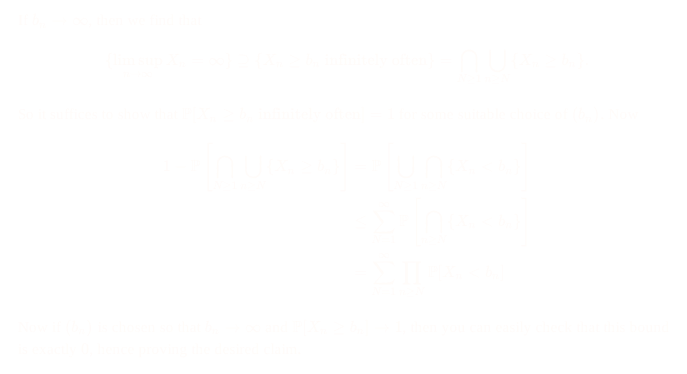
\includegraphics[width=.9\columnwidth]{figures/scott-tripos-in-the-wild.png}
% 		\end{center}
% 	\end{example}
% \end{frame}

% % \begin{frame}{Borel--Cantelli}
% % 	To convert the proof, we restate Borel--Cantelli for Scott triposes:

% % 	\begin{lemma}[1$^{st}$ Borel--Cantelli]
% % 		If $\{E_n\}_{n \in \N}$ are events s.t. $\sum_{n=1}^\infty \P(E_n) < \infty$ then
% % 		\begin{equation*}
% % 			\P(\limsup_n E_n) = 0
% % 		\end{equation*}
% % 	\end{lemma}

% % 	Becomes:

% % 	\begin{lemma}[1$^{st}$ Borel--Cantelli]
% % 		If $\varphi(n)$ is a ($W$-)predicate on $\N$ s.t. $\sum_{n=1}^\infty \P(\varphi(n)) < \infty$ then
% % 		\begin{equation*}
% % 			\Scott[W] \forces \exists n\; \forall k \geq n,\ \neg \varphi(k)
% % 		\end{equation*}
% % 	\end{lemma}
% % \end{frame}

% \begin{frame}{An example}
% 	To convert the proof, we restate Borel--Cantelli for Scott triposes:

% 	\begin{lemma}[2$^{nd}$ Borel--Cantelli]
% 		If $\{E_n\}_{n \in \N}$ are independent events s.t. $\sum_{n=1}^\infty \P(E_n) = \infty$ then
% 		\begin{equation*}
% 			\P(\limsup_n E_n) = 1
% 		\end{equation*}
% 	\end{lemma}

% 	Becomes:

% 	\begin{lemma}[2$^{nd}$ Borel--Cantelli]
% 		If $\varphi(n)$ is a ($W$-)predicate on $\N$ s.t. $\{n \in \N \suchthat \varphi(n)\}$ is an independent family and $\sum_{n=1}^\infty \P(\varphi(n)) = \infty$ then
% 		\begin{equation*}
% 			\Scott[W] \forces `\text{$\varphi(n)$ holds infinitely often}' %\forall n\; \exists k \geq n,\ \varphi(k)
% 		\end{equation*}
% 	\end{lemma}
% \end{frame}

% \begin{frame}{An example}
% 	We thus get the following `hybrid' proof:

% 	\vfill

% 	\begin{quotation}
% 		\noindent In the logic of $W$,
% 		\begin{equation*}
% 			`\text{$X_n \geq \sqrt{n}$ infinitely often}' \hey \limsup_n X_n = \infty
% 		\end{equation*}
% 		therefore it's sufficient to prove the first.

% 		\noindent If $X_n$ is uniformly distributed, then $\varphi(n) = `X_n \geq \sqrt{n}'$ are independent propositions and form a $W$-predicate on $\N$ such that
% 		\begin{equation*}
% 			\sum_{n=1}^\infty \P(\varphi(n)) = \sum_{n=1}^\infty (\underbrace{1-1/\sqrt{n}}_{= \frac1{2n} + o(1)}) = +\infty.
% 		\end{equation*}

% 		\noindent Hence the claim follows by 2$^{nd}$ Borel--Cantelli
% 	\end{quotation}

% 	\vfill
% \end{frame}

% \begin{frame}{Scott topos}
% 	Any tripos $\tripos T : \cat C^\op \to \Cat$ gives rise to a topos, its \textbf{Pitts topos} $\Pitts[T]$.

% 	\vfill

% 	\textbf{Idea}: we construct `sets' and `functions' using the logic of $\tripos T$.

% 	\vfill

% 	\begin{enumerate}
% 		\item Objects are pairs
% 		\begin{equation*}
% 			(X \tin \cat C,\ {\sim_X} \in \tripos T(X \times X))
% 		\end{equation*}
% 		where $\sim_X$ is a \textbf{partial} equivalence relation (PER)\\
% 		{\color{colorgold}$\qquad \rightsquigarrow$ `$x \sim_X x$' is thought of as `$x \in X$'}.
% 		\item Maps $(X, \sim_X) \to (Y, \sim_Y)$ are given by functional relations $F \in \tripos T(X \times Y)$. They compose as relations.
% 	\end{enumerate}

% 	\vfill

% 	Exponentials, limits and the s.o. classifier are built `as if' they were sets.

% 	%We denote by $\Delta X$ the discrete object $(X, =)$.
% \end{frame}

\begin{frame}{Tripos to topos}
	Since $\Scott[W]$ is localic, its associated topos can be presented as
	\begin{diagram*}
		\Sh \alg F \equi \Sh_\aetop \F \arrow[hook]{r} \&[-3ex] \Sh \F
	\end{diagram*}
	where `$\aetop$' is the almost-everywhere topology on $\F$:
	\begin{equation*}
		\text{$\{A_i\}_{i \in I}$ covers $A$}
		\sse
		\text{$\{A_i\}_{i \in I}$ `essentially covers' $A$}
	\end{equation*}

	\vfill
	\begin{definition}
		\begin{equation*}
			\Sh_\aetop W := \Sh \alg F \equi \Sh_\aetop \F \equi \Pitts[\Scott[W]]
		\end{equation*}
	\end{definition}

	\vfill
	It's the topos of `random sets and random functions' wrt to $W$.

	It's a classical universe: we have both LEM and AC.
\end{frame}


\begin{frame}{Geometry}
	We can look at this topos geometrically:

	\vfill
	\begin{center}
		\begin{tabularx}{\columnwidth}{C|c}
			\textbf{algebraic geometry} & \textbf{probability theory}\\[2ex]
			base scheme $S$ & base probability space $W$\\[2ex]
			regular functions & essentially bounded r.v.\\[2ex]
			structure sheaf $\O_S$ & `structure sheaf' $L^\infty(-,\R)$\\[2ex]
			commutative rings & commutative Von Neumann algebras\\
			& ({\color{colorgold} kind of})\\[2ex]
			Grothendieck topos $\Sh S$ & {\color{colorgold}Kolmogorov topos} $\Sh_\aetop W$
		\end{tabularx}
	\end{center}
	\vfill
\end{frame}

{
	\usebackgroundtemplate{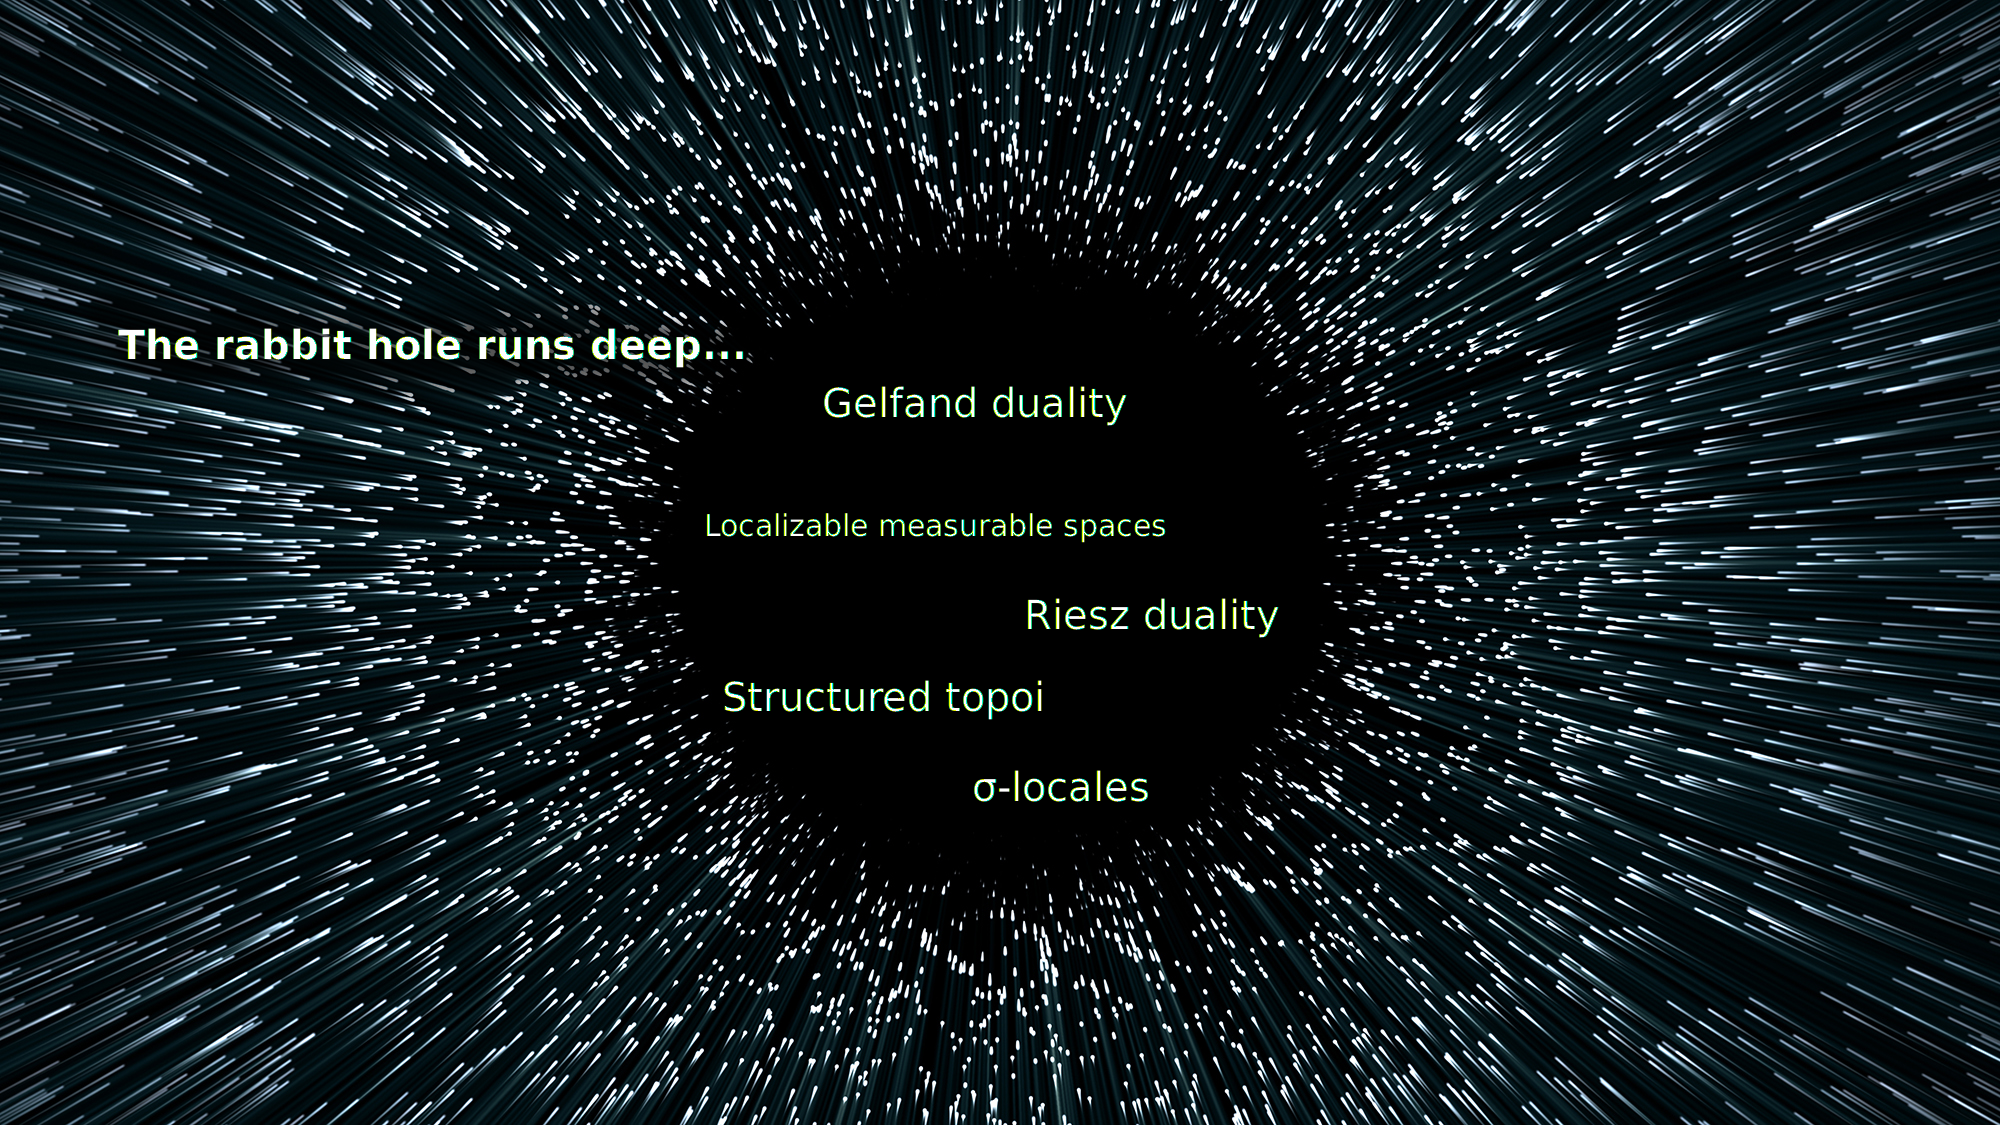
\includegraphics[height=\paperheight]{figures/blackhole.png}}
	\begin{frame}{Geometry}
	\end{frame}
}

\begin{frame}{Geometry}
	There is a \textbf{measurability structure}
	\begin{equation*}
		\O_W : \Msbl \to \Sh_\aetop W
	\end{equation*}
	given by \textbf{essential functors of points}
	\begin{equation*}
		\O_W(E) = \Msbl(-, E) / \underset{\aetop}{=}
	\end{equation*}
	and any null-reflecting map $f : W \to V$ induces a morphism
	\begin{diagram*}
		\Sh_\aetop W \&[-3ex] \&[-3ex] \Sh_\aetop V\\
		\& \Msbl
		\arrow[""{name=0, anchor=center, inner sep=0}, "{f_*}"', shift right=2, from=1-1, to=1-3]
		\arrow[""{name=1, anchor=center, inner sep=0}, "{f^*}"', shift right=2, from=1-3, to=1-1]
		\arrow["{\O_W}", from=2-2, to=1-1]
		\arrow[""{name=2, anchor=center, inner sep=0}, "{\O_V}"', from=2-2, to=1-3]
		\arrow["\dashv"{anchor=center, rotate=-90}, draw=none, from=1, to=0]
		\arrow[shorten <=20pt, shorten >=30pt, shift left=2, Rightarrow, from=2, to=1-1]
	\end{diagram*}
	\begin{equation*}
		f^*\O_V \longtwoto \O_W \quad\text{or, equivalently}\quad \O_V \longtwoto f_*\O_W
	\end{equation*}
\end{frame}

\begin{frame}{Internal notions}
	We can start looking for the objects of probability theory inside $\Sh_\aetop W$ (with the help of \cite{jackson2006sheaf}).
\end{frame}

\begin{frame}{Random variables}
	The internal real numbers are given by
	\begin{equation*}
		\RNO_W = \O_W(\R)
	\end{equation*}
	Hence this confirms `random variables' are indeed `variables' in a `random' setting.
	\vfill
	Then we can prove things like
	\begin{theorem}
		A sequence of random variables $\{X_n\}_{n \in \N}$ converges almost surely iff it converges in the usual sense as a sequence of internal real numbers.
	\end{theorem}
	\vfill
	Also, $L^p_{\color{colorgold}\mathsf{loc}}$ spaces become subsets of the real numbers.
\end{frame}

\begin{frame}{Integration}
	There's a sheaf $\M$ of measures on $W$, which is definable internally
	\begin{equation*}
		\M = \{ \mu \in \aetop(P\Q^+) \suchthat \text{$\mu$ is an `additive' upper cut}\}
	\end{equation*}
	Thus integration is straightforward: first, on simple rational functions:
	\begin{eqalign*}
		\int -\,\de - : \QNO^+ \times \M &\longto \M\\
		(q, \mu) &\longmapsto q \mu
	\end{eqalign*}
	then we extend by continuity:
	\begin{eqalign*}
		\int -\,\de - : \RNO^+ \times \M &\longto \M\\
		(X, \mu) &\longmapsto \underbrace{\bigvee_{q \leq X} q \mu}_{\color{colorgold}\int_{-} X\,\de\mu}
	\end{eqalign*}
	In particular, we defined $\Exp[X]$.
\end{frame}

\begin{frame}{Radon--Nikodym}
	Now recall

	\vfill
	\begin{theorem}[Radon--Nikodym]
		Let $\nu$ be a measure on $W$ such that $\mu(A) = 0$ implies $\nu(A) = 0$.
		Then there exists a positive measurable random variable $\der{\nu}{\mu}$ such that
		\begin{equation*}
			\int_{-} \der{\nu}{\mu} \, \de \mu = \nu(-)
		\end{equation*}
	\end{theorem}

	\vfill
	It says every absolutely continuous measure wrt $\mu$ has a $\mu$-density.
\end{frame}

\begin{frame}{Radon--Nikodym}
	We can prove the theorem internally (\cite{jackson2006sheaf}).
	Fix $\mu \tin \M$:
	\begin{enumerate}
		\item $\mu$-integration in an arrow $\int - \de \mu : \RNO^+ \to \M$.
		\item Its image $\M_{\int\!\mu}$ is contained in $\M^{\ll \mu}$, the object of absolutely continuous measures with respect to $\mu$.
		\item Then we want to show $\M_{\int\!\mu} = \M^{\ll \mu}$ so that $\der{-}{\mu}$ is the splitting of the image of $\int - \de \mu$:
		\begin{equation*}
			\der{-}{\mu} : \M^{\ll \mu} \longto \RNO^+
		\end{equation*}
	\end{enumerate}
	To do so, one fixes $\nu \tin \M^{\ll \mu}$ and defines
	\begin{equation*}
		\der{\nu}{\mu} = \bigvee \{q \in \QNO^+ \suchthat q \mu \leq \nu\}
	\end{equation*}
	up to technicalities, this concludes the proof!
\end{frame}

\begin{frame}{Martingales}
	For stochastic calculus, the most useful application of Radon--Nikodym is given by the definition of \textbf{conditional expectations}:
	\begin{definition}
		Given a filtration $\{F_t\}_{t \in I}$, the conditional expectation of $X$ at $t$ is defined as
		\begin{equation*}
			\Exp[X | \F_t] = \der{(\int X \, \de\P)\vert_{\F_t}}{\P\vert_{\F_t}}
		\end{equation*}
	\end{definition}
	%This is a $\F_t$-measurable r.v. representing the average of $X$ conditioned by the state of the world at time $t$.
	\begin{definition}
		A \textbf{martingale} is an adapted stochastic process such that
		\begin{equation*}
			\Exp[ X_{t+s} | \F_t] = X_t
		\end{equation*}
	\end{definition}
	It's a process not expected to change, e.g. the coin tosses bet, $B_t$.
\end{frame}

\begin{frame}{Internalizing martingales}
	To define a martingale internally we need

	\vfill
	\begin{enumerate}
		\item An internal definition of `stochastic process'
		\item An internal definition of `adaptedness' $\rightsquigarrow$ {\color{colorgold}filtrations}
		\item An internal definition of `conditional expectation at $t$'.
	\end{enumerate}

	\vfill
\end{frame}

\begin{frame}{Stochastic processes}
	\begin{theorem}
		An $E$-valued stochastic process $\{X_t\}_{t \in I}$ on $W$ corresponds to a map
		\begin{equation*}
			X:\Delta I \to \O_W(E)
		\end{equation*}
		in $\Sh_\aetop W$.
	\end{theorem}

	\vfill
	If $X$ is \textbf{measurable} as a map $W \times I \to E$, then this map can be lifted to
	\begin{equation*}
		X : \O_W(I) \to \O_W(E).
	\end{equation*}

	\vfill
	By extension, any map $X:I \to E$ in $\Sh_\aetop W$ is a `stochastic process'.

	% \vfill
	% The \textbf{law} of a real-valued stochastic process is the map
	% \begin{diagram*}
	% 	I \arrow{r}{X} \& \RNO \arrow{r}{\int - \de \P} \& \M
	% \end{diagram*}
	% Notice: I can distinguish between \textbf{versions} of the same process.
\end{frame}

\begin{frame}{Stochastic processes}
	Two facts:
	\vfill
	\begin{theorem}
		Two stochastic processes $X, Y : \Delta I \to \O_W(E)$ are equal in the logic of $\Sh_\aetop W$ iff they are \textbf{indistinguishable}, i.e.
		\begin{equation*}
			\P( \forall t \in I,\, X_t = Y_t) = 1
		\end{equation*}
		\vspace{-3ex}
	\end{theorem}

	Therefore we can state \& prove theorems like:

	\vfill
	\begin{theorem}
		A stochastic process is almost surely continuous iff it's continuous from the internal point of view.
	\end{theorem}
\end{frame}

% If X is not a measurable process

\begin{frame}{Filtrations}
	We need a way to express `\textit{measurability at $t$}' for elements in $\O_W(E)$.

	\vfill
	A filtration induces a chain of null-reflecting maps (each carried by $1_W$)
	\begin{equation*}
		W_\infty \longto \cdots \longto W_t \longto \cdots \longto W_0
	\end{equation*}
	where $W_t = (W, \F_t, \P\vert_{\F_t})$.

	\vfill
	which in turn becomes a chain of (surjections of) Kolmogorov topoi:\\
	\begin{diagram*}
		\Sh_\aetop W_\infty
			\arrow[shift right=2, swap]{r}
		\&[-1ex]
		\cdots
			\arrow[shift right=2, swap, hook, "\perp"{below}]{l}
			\arrow[shift right=2, swap]{r}
		\&[-1ex]
		\Sh_\aetop W_t
			\arrow[shift right=2, swap, hook, "\perp"{below}]{l}
			\arrow[shift right=2, swap]{r}
		\&[-1ex]
		\cdots
			\arrow[shift right=2, swap, hook, "\perp"{below}]{l}
			\arrow[shift right=2, swap]{r}
		\&[-1ex]
		\Sh_\aetop W_0
			\arrow[shift right=2, swap, hook, "\perp"{below}]{l}
	\end{diagram*}
\end{frame}

\begin{frame}{Filtrations}
	Remember that null-reflecting maps induce maps
	\vspace{-4ex}
	\begin{center}
		\Large
		\begin{diagram*}
			\Sh_\aetop W_\infty \&[-3ex] \&[-3ex] \Sh_\aetop W_t\\
			\& \Msbl
			\arrow[""{name=0, anchor=center, inner sep=0}, "{{1_t}_*}"', shift right=2, from=1-1, to=1-3]
			\arrow[""{name=1, anchor=center, inner sep=0}, "{1_t^*}"', hook, shift right=2, from=1-3, to=1-1]
			\arrow["{\O_\infty}", from=2-2, to=1-1]
			\arrow[""{name=2, anchor=center, inner sep=0}, "{\O_t}"', from=2-2, to=1-3]
			\arrow["\dashv"{anchor=center, rotate=-90}, draw=none, from=1, to=0]
			\arrow[shorten <=20pt, shorten >=30pt, shift left=2, Rightarrow, from=2, to=1-1]
		\end{diagram*}
	\end{center}

	\vfill
	Hence for every $t \in I$, $E \tin \Msbl$, we have
	\begin{equation*}
		1_t^*\O_t(E) =: \O_t^*(E) \longto \O_\infty(E)
	\end{equation*}
\end{frame}

\begin{frame}{Filtrations}
	The inclusion $\alg F_t \into \alg F_\infty$ has both adjoints, in particular
	\begin{eqalign*}
		1_t^{-1} \dashv \lozenge_t : \alg F_\infty &\longto \alg F_t\\
						A	&\longmapsto \bigwedge \{B \in \F_t \suchthat A \leq B \}
	\end{eqalign*}
	{\color{colorgold}We can interpret it as a `\textit{possibly at $t$}' modal operator.}

	\vfill
	Thus for each $A \in \alg F_\infty$:
	\begin{equation*}
		\O_t^*(E)(A) := \O_t(E)(\lozenge_t A) = \Msbl(\lozenge_t A, E) / \underset{\aetop}{=}
	\end{equation*}
	and
	\begin{eqalign*}
		\O_t^*(E)(A) &\longto \O_\infty(E)(A)\\
		{\color{colorgold}\lozenge_t A \nto{f} E} &\longmapsto {\color{colorgold}A \into \lozenge_t A \nto{f} E}
	\end{eqalign*}
	Notice: $\lozenge_t A \subseteq W_t$, while $A \subseteq W_\infty$\\
	\hspace*{3ex} {\color{colorgold}$\rightsquigarrow$ $\O^*_t(E)$ contains $\F_t$-measurable elements}.
\end{frame}

\begin{frame}{Filtrations}
	For each $t \in I$, let {\color{colorgold}$\msbl(t)$} be the image of $\O_t^*(E)$ in $\O_\infty(E)$.\\[1ex]
	Sheafification extends this definition: given $\tau \tin \Delta I$,
	\begin{equation*}
		W \forces e \in \msbl(\tau) \sse \text{for all $s \in I$, $\{\tau = s\} \forces e \in \msbl(s)$}
	\end{equation*}

	\vfill
	\begin{diagram*}
		\mathsf{const}(I) \arrow{dr}{\msbl} \arrow[swap]{d}{\eta_\aetop}\\
		\Delta I \arrow[dashed]{r}{\msbl} \& P\O_\infty(E)
	\end{diagram*}

	\vfill
	We can extend the definition of $\msbl$ to $\O_\infty(I)$:
	\begin{equation*}
		W \forces \forall \tau \tin \O_\infty(I),\ \msbl(\tau) \Leftrightarrow \forall \sigma \tin \Delta I,\ \sigma \leq \tau \hey \msbl(\sigma)
	\end{equation*}
	This recovers $\F_\tau$-measurability for a \textbf{random time} $\tau : W \to I$.
\end{frame}

\begin{frame}{Filtrations}
	\begin{definition}
		We call $X:\Delta I \to \O_\infty(E)$ \textbf{adapted} iff
		\begin{equation*}
			W \forces \forall t \tin \Delta I,\ X(t) \in \msbl(t)
		\end{equation*}
	\end{definition}

	% \vfill
	\begin{theorem}
		External adaptedness coincides with internal adaptedness
	\end{theorem}

	\vfill
	\begin{block}{Open question}
		Is there a better \textbf{internal/synthetic} notion of adaptedness?
	\end{block}

	\vfill
	\textbf{Alternative construction} suggested by Morgan Rogers (priv. comm.):
	\begin{enumerate}
		\item The object $\F_\bullet = \{\F_t\}_{t \in I}$ is naturally in $\Psh (I, \leq)$
		\item Adapted processes are maps of internal sheaves over $\F_\bullet$!
	\end{enumerate}
\end{frame}

% \begin{frame}{Filtrations}
% 	Notice that there's a morphism
% 	\begin{diagram*}
% 		\lozenge_t : \Omega_\infty \arrow{r} \& 1_t^* \Omega_t \arrow{r} \& \Omega_\infty\\[-7ex]
% 		\text{$B \leq A$} \arrow[mapsto]{r} \& \text{$\lozenge_t B \leq \lozenge_t A$} \arrow[mapsto]{r} \& \text{$A \cap \lozenge_t B \leq A$}
% 	\end{diagram*}
% 	Even easier using $\Scott[W]$:
% 	\begin{eqalign*}
% 		\lozenge_t : \alg F_\infty \times \alg F_\infty &\longto \alg F\\
% 					(A, B)			&\longmapsto \lozenge_t A \Leftrightarrow B
% 	\end{eqalign*}

% 	\vfill
% 	Let $\Phi_t$ be the image of $\lozenge_t$, for every $E \tin \Sh_\aetop W$ we can define
% 	\begin{equation*}
% 		\varphi_t^E = \{ \psi \in PE \suchthat \forall e \tin E,\ \psi(e) \in \Phi_t \}
% 	\end{equation*}

% 	\begin{theorem}
% 		\begin{equation*}
% 			W \forces z \in \msbl(t) \Leftrightarrow z = z \in \phi_t^{\O_W(E)}
% 		\end{equation*}
% 	\end{theorem}
% \end{frame}

\begin{frame}{Conditional expectation}
	Restrictions of measures is given by the canonical inclusion
	\begin{diagram*}
		{1_t}_*\M_\infty \arrow[hook]{r}{-\vert_t} \& \M_t
	\end{diagram*}
	Then we define
	\begin{diagram*}
		\Exp[- | \F_t]_t = {1_t}_*\RNO^+_\infty \arrow{r}{(\int - \de \P)\vert_t} \& \M^{\ll \P\vert_t} \arrow{r}{\der{}{\P\vert_t}} \& \RNO^+_t
	\end{diagram*}
	Finally:
	\begin{diagram*}
		\Exp[- | \F_t]_\infty := \RNO^+_\infty
			\arrow{r}{\text{ext. by 0}}
		\& 1_t^* {1_t}_* \RNO^+_\infty
			\arrow{r}{1_t^* \Exp[X \vert \F_t]_t}
		\& 1_t^*\RNO^+_t
			\arrow{r}{A \into \lozenge_t A}
		\&[-1ex] \RNO^+_\infty
	\end{diagram*}

	If we unpack the definitions, this is what's happening (hand-wavingly):
	\begin{eqalign*}
		X &\mapsto %{\bigvee \{q_t \in \QNO^+_t \suchthat q_t \P_t \leq (\bigvee \{q_\infty \P \in \Q_\infty^+ \suchthat q_\infty \leq X\})_t}\\
		\bigvee \{q_t \in 1_t^*\QNO^+_t \suchthat q_t \leq ({\textstyle \int} X\,\de \P) / \P\}
	\end{eqalign*}
	\begin{center}
		{\color{colorgold}best approximation at $t$ of $X$'s average}.
	\end{center}
\end{frame}

\begin{frame}{Martingales, finally}
	\begin{definition}
		A map $X : \Delta I \to \O_\infty(E)$ is a \textbf{martingale} if it is adapted and
		\begin{equation*}
			W \forces \forall t \tin \Delta I\,\, \forall s \geq t,\ \Exp[X(t+s) | \F_t]_\infty = X(t),
		\end{equation*}
	\end{definition}
\end{frame}

	% \begin{frame}{What's missing}
% 	\begin{enumerate}
% 		\item Stopping times
% 		\item Convergence in probability
% 		\item Stochastic calculus!
% 	\end{enumerate}
% \end{frame}

% \begin{frame}{Outro}
% 	Recapping...
% 	\begin{enumerate}
% 		\item There's a topos theory $\Sh_\aetop W$ which embodies 'randomness over $W$'\\
% 		$\rightsquigarrow$ {\color{colorgold}too stubborn to see the quantitative (`linear') aspects}
% 		\item There are topoi $\Sh_\aetop W$ which mimick the Grothendieck topoi of schemes\\
% 		$\rightsquigarrow$ {\color{colorgold} how far does the analogy go?}
% 		\item The probabilist's habit of considering random variables `elements'/`numbers' and stochastic processes `maps' is well-founded\\
% 		\item We can (clumsily) use filtrations and define conditional expectations\\
% 		$\rightsquigarrow$ {\color{colorgold}TODO: go all the way to stochastic calculus}
% 	\end{enumerate}
% \end{frame}

\begin{frame}{Roadmap}
	
\includegraphics[width=\columnwidth]{figures/roadmap.png}
\end{frame}


	\begin{framecard}
		{\color{white}
		\bfseries

		\hugetext{Thanks for your attention!}
		\largetext {Questions?}}
	\end{framecard}

	\begin{frame}[allowframebreaks]{References}
		\nocite{*}
		\printbibliography
	\end{frame}
\end{document}
